\documentclass{article}
\usepackage[utf8]{inputenc}
\usepackage{siunitx}
\usepackage{graphics}
\usepackage[american,siunitx]{circuitikz}
\usepackage{amsmath}
\usepackage{svg}
\usepackage{booktabs}
\usepackage{float}
\usepackage{xparse, xfp}
%\renewcommand{\thesubsection}{\thesection.\alph{subsection}}
\newcommand{\equal}{=}
\ExplSyntaxOn
\NewDocumentCommand{\defcon}{mm}
 {
  \cs_new:Npx #1 { \fp_eval:n { #2 } }
 }
\ExplSyntaxOff

\title{ECE2101L\\Electrical Circuit Analysis II Laboratory\\\,\\Lab 3\\Time Constants of First Order RC Circuits\\\,\\Prelab\\}
\author{Choi Tim Antony Yung}
\date{17 February 2020}

\begin{document}

\maketitle

\newpage

%1
\section{Natural Response of First Order RC Circuit}

\begin{center}
    \begin{circuitikz}
        \draw 
            (0,0) to[C, l_=C,i>_=$i_C$] (0,-2)
            (0,0) -- (1,0) node[circle,draw=black,inner sep=0pt,fill=white,minimum size=3pt]{} -- (2,0)
            to[R=R, i>^=$i_R$] ++(0,-2) -- (1,-2) node[ground]{} -- (0,-2)
            (1.25,-0.25)to[open,v=v](1.25,-1.75)
            ;
    \end{circuitikz}
\end{center}

%1.1
\subsection{For the above RC circuit:}
$$i_C=C\frac{dv_c}{dt}=C\frac{dv}{dt}$$
$$i_R=\frac{V_R}{R}=\frac{v}{R}$$
$$i_C+i_R=0$$
\null\hfill ... from KCL
$$C\frac{dv}{dt}+\frac{v}{R}=0$$
$$\frac{dv}{dt}=-\frac{1}{RC}v$$
$$\int \frac{1}{v}\, dv=\int -\frac{1}{RC} \, dt$$
$$ln(v)=-\frac{t}{RC}+C$$
\null\hfill ... where C is a constant
$$v=e^{-\frac{t}{RC}+C}=e^Ce^{-\frac{t}{RC}}$$
$$v(0)=e^Ce^{-\frac{0}{RC}}=e^C=V_0$$
$$v(t)=V_0e^{-t/RC}$$

%1.2
\subsection{RC in the above equation is the time constant of the RC circuit. It determine how fast the capacitor discharges.}

%1.3
\subsection{The equation above describe the voltage response of an RC circuit in the absence of an external input, hence the term "natural" response.}

\pagebreak

\section{Thevenin Equivalent Resistance}
\begin{center}
    \begin{circuitikz}
        \draw
            (0,0) to[R,l_=\SI{7}{\ohm}]++(0,-3)
            (1.5,0) to[R,v^=$v_x$,l_=\SI{6}{\ohm}]++(0,-3)
            (0,0) -- (1.5,0) to[R=\SI{15}{\ohm},i>^=$i_o$] ++(3,0)
            to[C=$\frac{1}{3}$F, v=$v_C$] ++(0,-3) -- (0,-3)
            ;
    \end{circuitikz}
\end{center}

\subsection{The Thevenin equivalent resistance at the capacitor terminal can be determined as follow:}
$$\frac{1}{\frac{1}{7}+\frac{1}{6}}+15=\SI{18.2308}{\ohm}$$

\subsection{The equivalent circuit can then be derived:}
\begin{center}
    \begin{circuitikz}
        \draw
            (0,0) to[R,l_=\SI{18.2308}{\ohm}]++(0,-3)
            (0,0) to[short] ++(3,0)
            to[C=$\frac{1}{3}$F, v=$v_C$] ++(0,-3) -- (0,-3)
            ;
    \end{circuitikz}
\end{center}

\section{Time to Reach the Steady State}
\begin{center}
	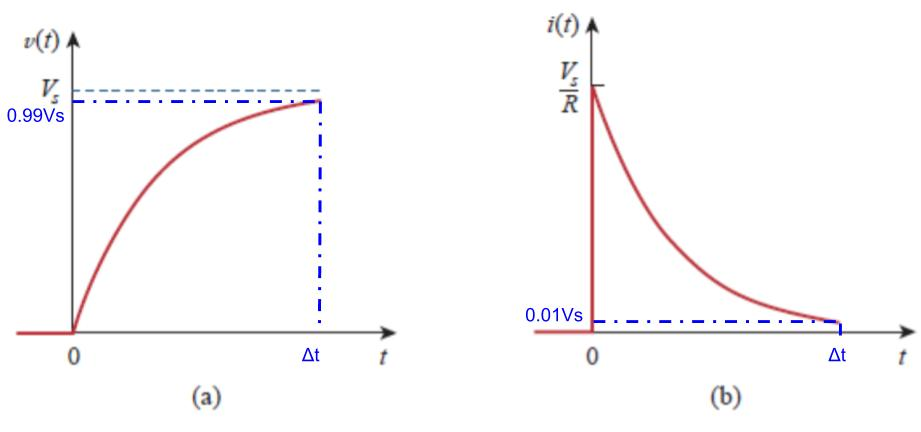
\includegraphics[scale=0.35]{drawing.jpg}
\end{center}

\pagebreak

\section{Pulse Waveform Generation}
According to the Quick Start section of the Keysight 33210A waveform generator service guide, a pulse waveform can be generated by the following procedure: Turn on the power by pressing the power button, press the "Pulse" key to set the output waveform as pulse waveform, press the soft key and turn the knob to set the value for required parameter: Frequency (Freq) or Period, Amplitude (Ampl), DC Offset (Offset), Pulse Width (Width) and Edge Time. The waveform output will start after connecting the Output BNC socket and the circuit and hitting the Output button.\\
\\
In the absence of Keysight 33210A waveform generator, the Tektronix FG 503 Function Generator can be use to generate square wave to simulate pulse waveform with the disadvantage that period must be twice the width of the pulses and there are no setting for edge time. According to the Instruction Manual of FG 503, the rise time (edge time) of the square wave is less than or equal to 60ns.


\end{document}